\documentclass[
    paper=a4,               % paper format
    fontsize=10pt,          % fontsize
    %twoside,               % double-sided
    open=right,             % begin new chapter on right side
    titlepage=false,        % use no standard title page
    parskip=half,           % set paragraph skip to half of a line
]{scrreprt}                 % KOMA-script report

\raggedbottom{}

% Load Standard Packages:
%---------------------------------------------------------------------------
\usepackage{scrpage2}
\usepackage[standard-baselineskips]{cmbright}
\usepackage[ngerman]{babel}                                             % german hyphenation
\usepackage[utf8]{inputenc}                                             % UTF-8 character encoding
\usepackage[T1]{fontenc}                                                % hyphenation of words with ä,ö and ü
\usepackage{textcomp}                                                   % additional symbols
\usepackage{ae}                                                         % better resolution of Type1-Fonts 
\usepackage{etoolbox}                                                   % color manipulation of header and footer
\usepackage{graphicx}                                                   % integration of images
\usepackage{float}                                                      % floating objects
\usepackage{caption}                                                    % for captions of figures and tables
\usepackage{booktabs}                                                   % package for nicer tables
\usepackage{tocvsec2}                                                   % provides means of controlling the sectional numbering
\usepackage[square,sort,comma,numbers]{natbib}                          % provides various citation styles
\usepackage{wrapfig}                                                    % provides floating of text around images
\usepackage{nameref}                                                    % provides printing names of references
\usepackage{multicol}                                                   % Foo
\usepackage{subcaption}
%---------------------------------------------------------------------------

%---------------------------------------------------------------------------
% Set up page dimension
%---------------------------------------------------------------------------
\usepackage{geometry}
\geometry{a4paper,
    left=28mm,
    right=15mm,
    top=5mm,
    headheight=5mm,
    headsep=0mm,
    textheight=282mm,
    footskip=5mm
}
%---------------------------------------------------------------------------

\begin{document}

    \chapter*{Semantische Datenbanken}

    Computer Perception and Virtual Reality / Prof.\ Dr.\ Jürgen Eckerle\\
    Experte: Jean-Marie Leclerc

    % Lead: 480
    \textbf{Der klassische Ansatz der Wissensabbildung, zum Beispiel in Form von UML, welchem die relationale Datenspeicherung zugrunde liegt, wird in der heutigen Informatik weitläufig eingesetzt und ist de facto Standard. Häufig geschieht dies in enger Verbindung mit der objektorientierten Programmierung. Experten aus einer Fachrichtung sind fähig, die Daten zu interpretieren und Schlüsse zu ziehen. Es ist damit aber nicht möglich Fragestellungen zu beantworten, welche über reine Relationsverknüpfungen hinausgehen. Mit dieser Technik sind Objekteigenschaften und -verhalten schwer abbildbar. Semantische Datenbanken sind eine andere Art Wissen zu repräsentieren. Sie ermöglichen das Abbilden von Objekteigenschaften und können mithilfe von Schlussfolgerungen die Rolle eines Experten einnehmen.}

    % Text: 2400
    \begin{multicols}{3}
        \section*{Wissenabbildung}
        Semantische Datenbanken werden auf der Basis von \textbf{Ontologien} erstellt. Eine Ontologie beschreibt Sachwissen einer Wissens- bzw. Problem-Domäne. Sie wird überall dort verwendet, wo Semantik zur Formulierung von Informationen benutzt wird. Ontologien werden in Form von \textbf{Tripeln} abgelegt. Tripel beinhalten \textit{Subjekt, Prädikat} und \textit{Objekt}. Zum Beispiel \textit{Seilpark hatStandort Balmberg}. So können Objekte und deren Eigenschaften sowie Beziehungen zwischen Objekten abgebildet werden.

        Die Verwendung von \textbf{Regeln} ist eine weitere Komponente der Wissensabbildung. Diese ermöglichen es Schlüsse zu ziehen. So kann beispielsweise definiert werden, dass eine Reise \textit{aufregend} (actionreich) ist, wenn sie \textit{Mut erfordert}.

        Aufgrund der Wissensbasis, bestehend aus Ontologie und Regeln, können mithilfe eines \textbf{Reasoners} (Inferenz-Maschine) Schlüsse gezogen werden.
        Ein \textbf{Reasoner} ist eine Software-Komponente, welche mittels Inferenz und Resolution zusätzliches Wissen ableiten kann. Hierfür wird \textbf{Beschreibungslogik} (ein Teil der Prädikatenlogik) benützt.

        {[}Inferenz: Aufbereitetes Wissen, das aufgrund von logischen Schlussfolgerungen gewonnen wurde.\\
        Resolution: Verfahren der formalen Logik, um eine logische Formel auf Gültigkeit zu testen.{]}

        \section*{Aufgabenstellung und Umsetzung}
        Ziel dieser Arbeit:  Aufbau einer semantischen Datenbank anhand einer konkreten Wissensdomäne.  Nutzung dieser Datenbank. Weiter soll gezeigt werden, wie ein Knowledge Engineer bei der Wissensmodellierung durch Ontologien vorgehen kann.

        Konkret wurde Reiseplanung als Wissensdomäne gewählt. In der heutigen Zeit werden Urlaubsaufenthalte/Pauschalreisen häufiger über Internet gebucht. Wenn jedoch ein Kunde spezielle Wünsche hat, so muss er sich immer noch in einem Reisebüro beraten lassen. 

        Um eine sehr individuelle Reiseplanung zu erreichen, musste zuerst eine Ontologie in Form von Klassen, Individuen, Relationen, Eigenschaften und Regeln erstellt werden. Ohne klaren Rahmen würde eine Ontologie zu komplex und zu gross. Daher wurde die Ontologie anhand exemplarischer Reisen schrittweise aufgebaut.

        Um auf gespeichertes Fachwissen einer Ontologie zugreifen zu können, werden Kenntnisse der Ontologie und Beherrschung einer speziellen Abfragesprache benötigt.

        Um eine benutzerfreundliche Reiseplanung zu bieten, wurde eine Webapplikation zur Reiseplanung entwickelt. Diese ermöglicht das Planen einer Reise mithilfe eines Assistenten. Der Benutzer kann die gewünschten Reisekriterien auswählen. Er erhält eine Auswahl an Reiseobjekten, welche seinen Kriterien entsprechen.

       Der theoretische Teil der Arbeit beinhaltet ein Tutorial, das aufzeigt, wie man bei Aufbau und Nutzung eines Expertensystems schrittweise vorgehen kann.

    \end{multicols}

    \begin{figure}[htbp]
        \begin{minipage}[hbt]{0,49\textwidth}
            \centering
            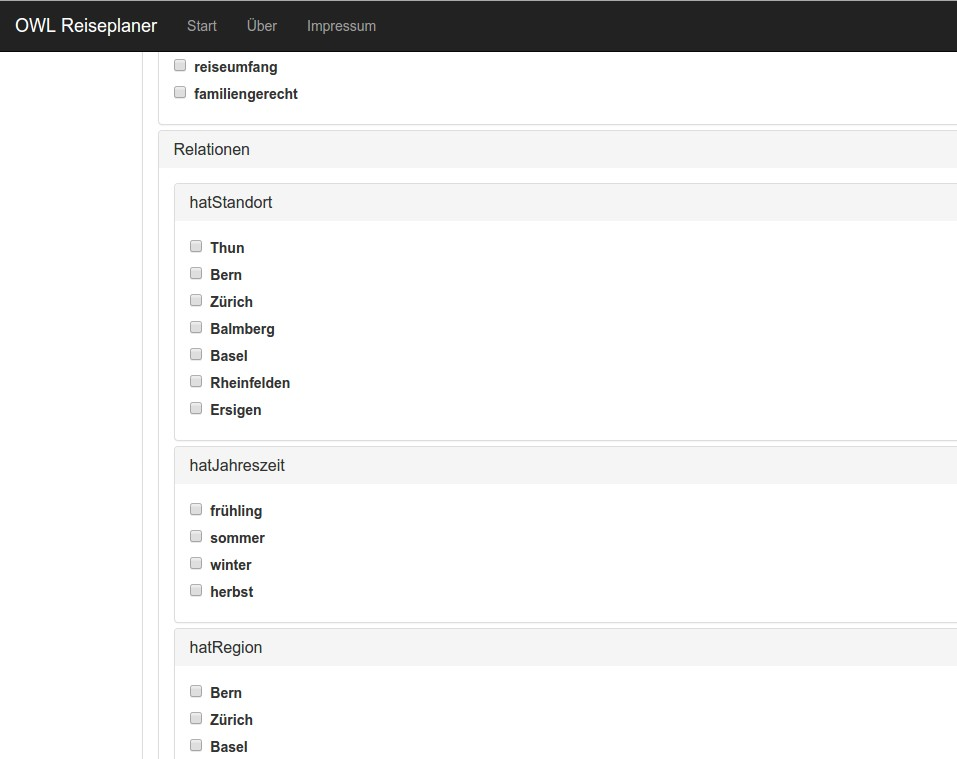
\includegraphics[scale=0.3]{bilder/reiseplaner_gui.jpg}
            \caption*{Benutzeroberfläche des Reiseplaners}
        \end{minipage}
        \begin{minipage}[hbt]{0,49\textwidth}
            \centering
            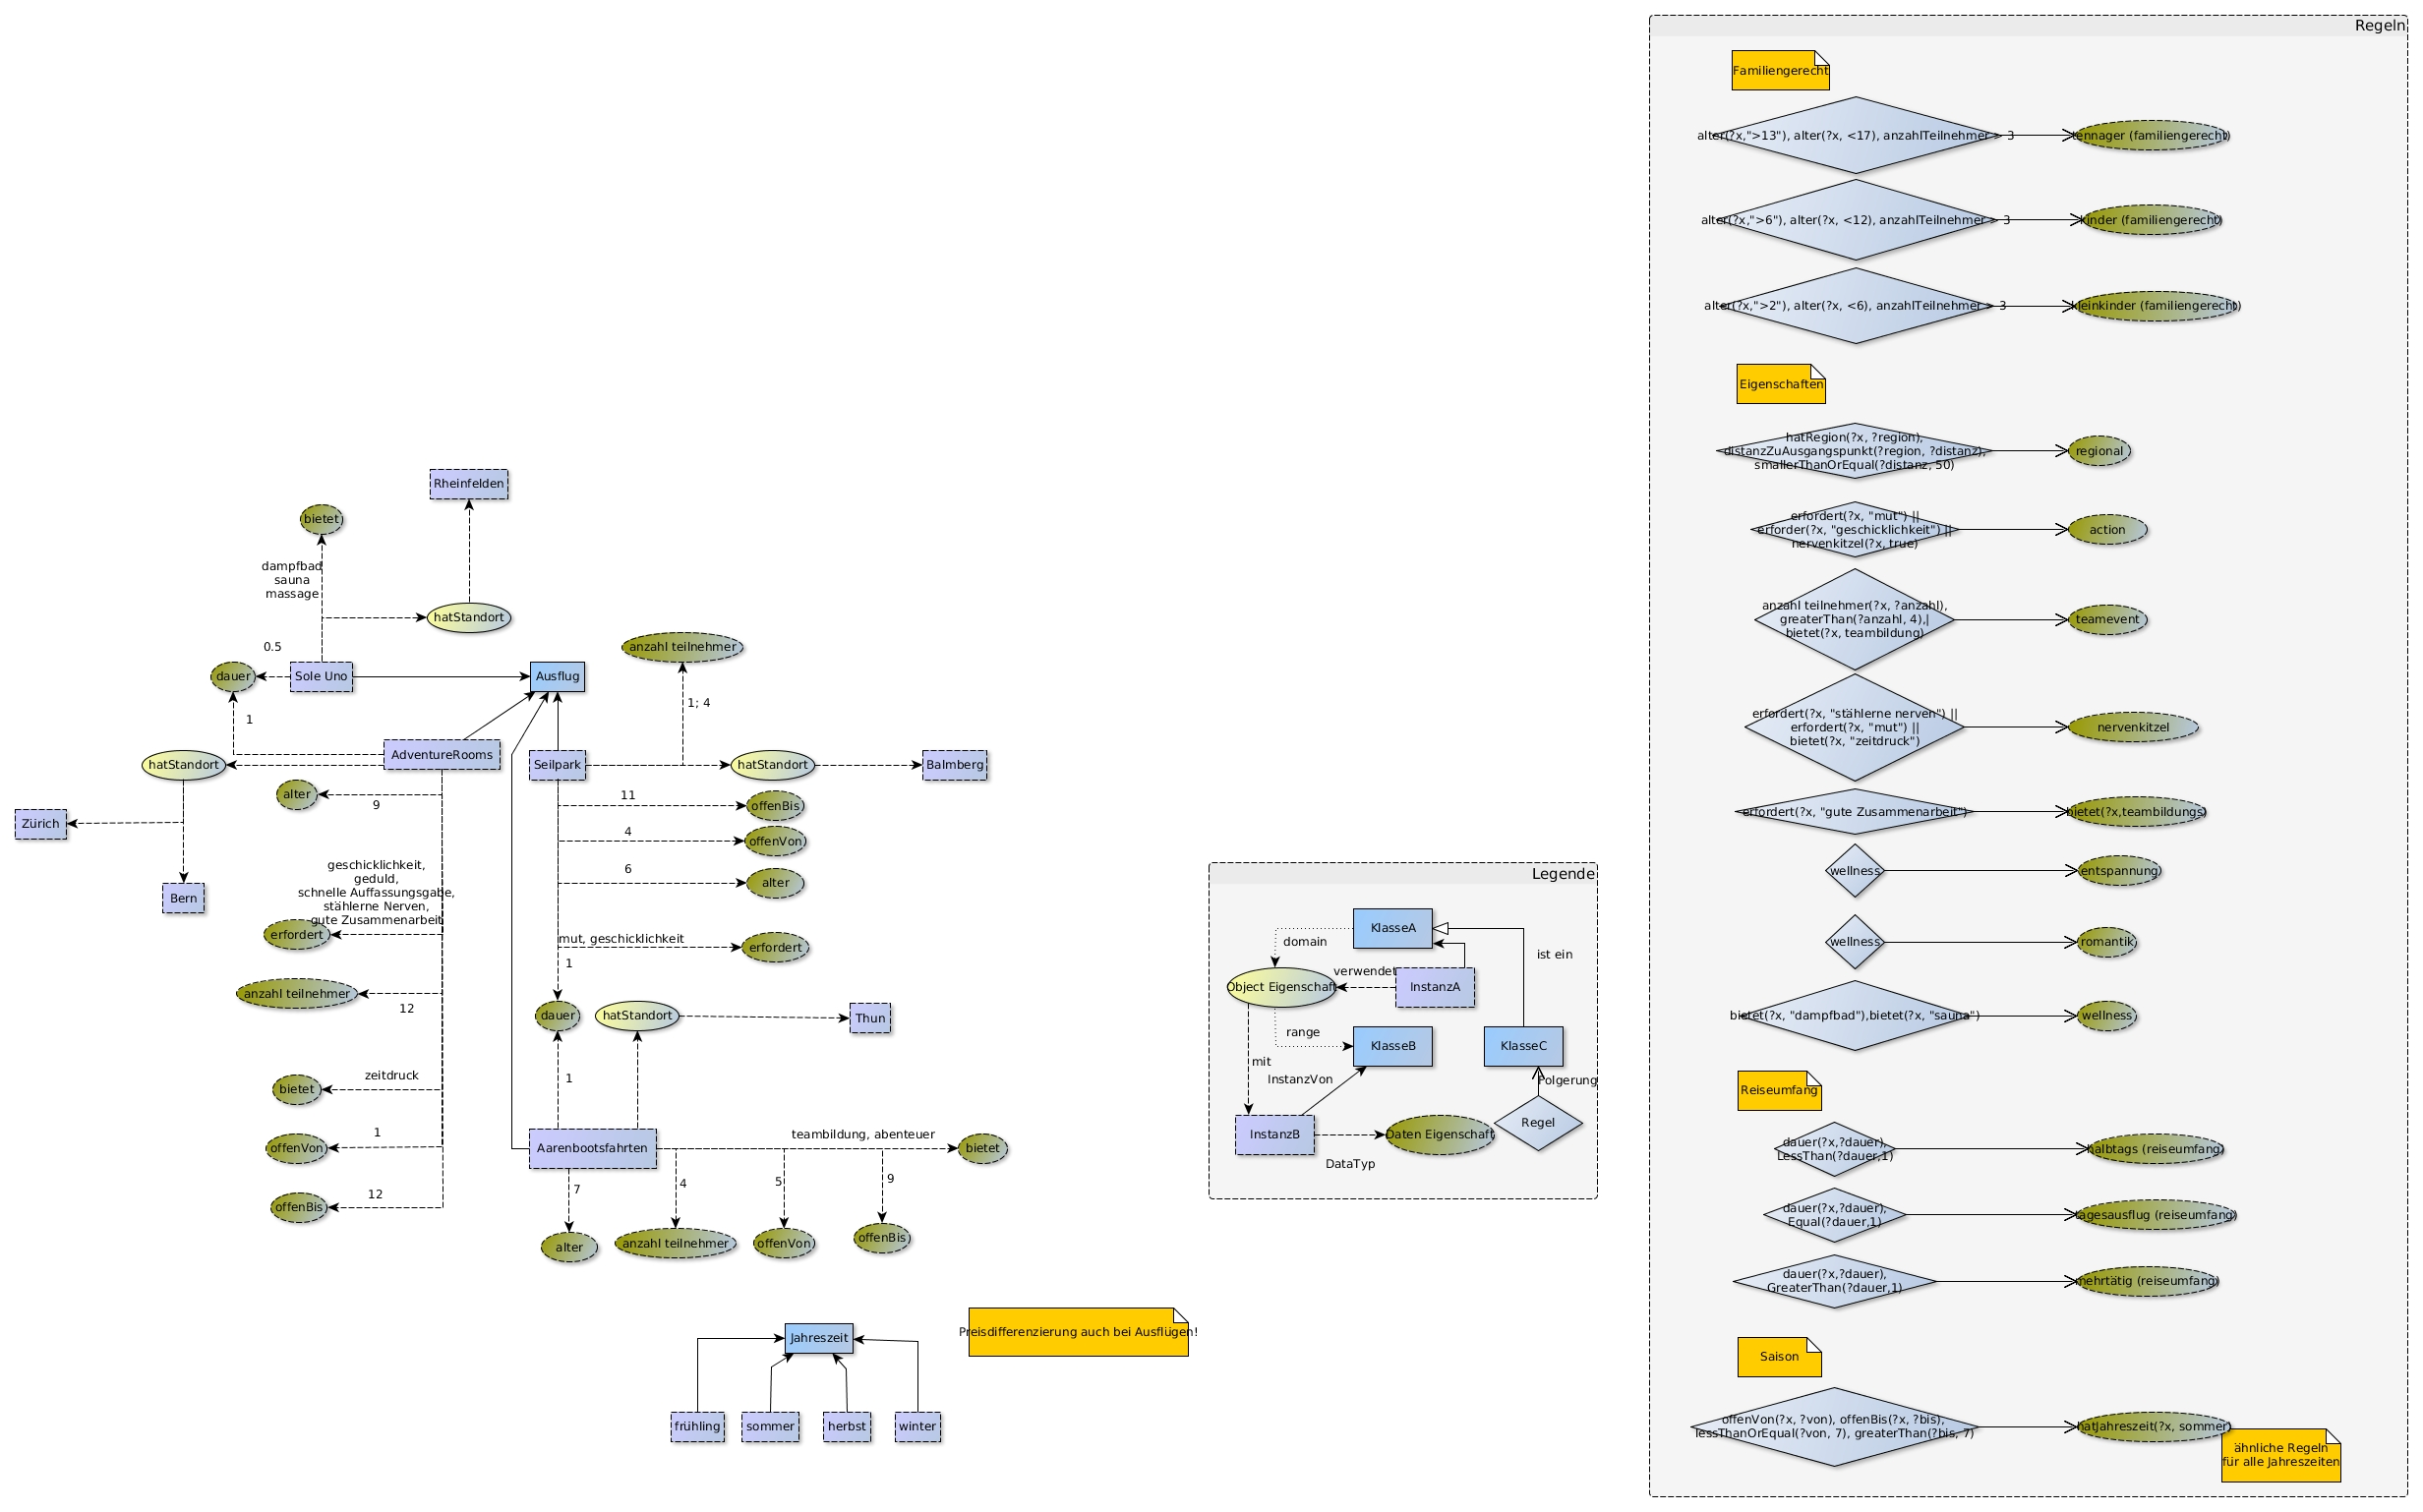
\includegraphics[scale=0.3]{bilder/semantisches_netz.jpg}
            \caption*{Reiseplaner als semantisches Netz}
        \end{minipage}
    \end{figure}
\end{document}
